\begin{XeClass}{FsConfig}
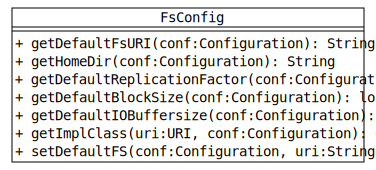
\includegraphics[width=10cm]{cdig/FsConfig.png}
     
 这个类保存了文件相关的一些Key,并且对外提供简单的借口,
 来实现设置或者获取Configuration对象的内容

    \begin{XeMethod}{\XePublic}{String}{getDefaultFsURI}
         
 获取默认的文件系统路径

    \end{XeMethod}

    \begin{XeMethod}{\XePublic}{String}{getHomeDir}
         
 获取文件系统的home文件目录

    \end{XeMethod}

    \begin{XeMethod}{\XePublic}{short}{getDefaultReplicationFactor}
         
 获取默认的文件副本数量

    \end{XeMethod}

    \begin{XeMethod}{\XePublic}{long}{getDefaultBlockSize}
         
 获取默认的文件块的大小

    \end{XeMethod}

    \begin{XeMethod}{\XePublic}{int}{getDefaultIOBuffersize}
         
 获取默认的Buffer的大小

    \end{XeMethod}

    \begin{XeMethod}{\XePublic}{Class<?>}{getImplClass}
         
 获取文件Scheme对应的类

    \end{XeMethod}

    \begin{XeMethod}{\XePublic}{void}{setDefaultFS}
         
 Setters: 功能都对应上面的Getters

    \end{XeMethod}

\end{XeClass}
